\documentclass[manuscript]{aastex}
\usepackage{booktabs}

\usepackage{natbib}
\bibliographystyle{apj}
\newcommand{\vdag}{(v)^\dagger}
\newcommand{\myemail}{daughjd@gatech.edu}

%\slugcomment{}
\shorttitle{Short Neutrino Transients in DeepCore-IceCube}
\shortauthors{IceCube et al.}

%% This is the end of the preamble.  Indicate the beginning of the
%% paper itself with \begin{document}.

\begin{document}

%% LaTeX will automatically break titles if they run longer than
%% one line. However, you may use \\ to force a line break if
%% you desire.

\title{Search for Short Transient Neutrino Emission with DeepCore-IceCube}
\author{IceCube Authors}
%% Use \author, \affil, and the \and command to format
%% author and affiliation information.
%% Note that \email has replaced the old \authoremail command
%% from AASTeX v4.0. You can use \email to mark an email address
%% anywhere in the paper, not just in the front matter.
%% As in the title, use \\ to force line breaks.

\begin{abstract}
We present the results of a search for sources of brief transient neutrino emission using IceCube and DeepCore data acquired between May 15th 2012 and April 30th 2013. While the search methods employed in this analysis are similar to those used in previous IceCube point source searches, the data set being examined consists of a sample of predominantly sub-TeV muon neutrinos obtained through a novel event selection method. Thus, this search represents a first attempt at identifying astrophysical neutrino sources in this relatively unexplored energy range. The reconstructed direction and time of arrival of neutrino events is used to search for any significant self-correlation in the dataset; there is no comparison of the data set to a list of possible sources. This search encompasses the Northern sky ranging in declination from -5$^{\circ}$ to 90$^{\circ}$. Examination of the data revealed no significant source of transient neutrino emission. This result has been used to construct limits on generic soft-spectra transients as well as a specific model of neutrino emission from soft jets in core-collapse supernovae.
\end{abstract}

%% Keywords should appear after the \end{abstract} command. The uncommented
%% example has been keyed in ApJ style. See the instructions to authors
%% for the journal to which you are submitting your paper to determine
%% what keyword punctuation is appropriate.

\keywords{neutrino astronomy, neutrinos, GRB, supernova, astroparticle physics}


\section{Introduction}
The nascent field of neutrino astronomy exhibits great potential in its ability to answer several open questions in astrophysics. This is largely due to the ability of the neutrino to probe the densest regions of astrophysical environments. Specifically, the detection of transient astrophysical neutrino sources will help shed light on the acceleration mechanisms at work in some of the most energetic phenomena in the Universe such as gamma-ray bursts, supernovae, and active galactic nuclei.

The detection of astrophysical neutrino sources is a chief goal of the IceCube Neutrino Observatory \citep{2006APh....26..155I}. Located at the geographic South Pole, IceCube utilizes the clear glacial ice of the Antarctic ice cap as a detection medium for the secondary products of neutrino interactions. The detector consists of 5,160 Digital Optical Modules (DOMs) distributed among 86 cables to form a km$^3$ instrumented volume. These DOMs house photomultiplier tubes for the capture of Cherenkov photons as well as digitizing electronics for initial processing of the PMT data. A centrally located region of denser instrumentation featuring DOMs with more sensitive PMTs comprises the sub-array DeepCore \citep{2012APh....35..615A}. This extension to IceCube array augments the detector's response to lower energy neutrino events.

IceCube analyses attempting to resolve astrophysical neutrino sources typically make use of a high-energy muon neutrino sample ($E_{\nu} \gtrsim 1$ TeV) of high-purity to look for both steady \citep{2014ApJ...796..109A} and transient sources \citep{2015arXiv150300598A}. As of yet, these searches have not found any significant self-correlations within the data sample nor correlations between the neutrino data and known astrophysical objects of interest. These analyses have largely eschewed low energy neutrino events collected by DeepCore due to poor resolution of these events as well as an increasingly strong irreducible background at lower energies given by the soft spectrum of atmospheric neutrinos. However, application of these predefined search techniques to a sample of low energy (30 GeV $\leq E_{\nu} < 1$ TeV) muon neutrino events from DeepCore can enhance IceCube's sensitivity to short transient neutrino sources with softer spectra.

Because of the strong atmospheric neutrino background in this energy range, searches using a data set composed of these low energy events will only be sensitive to time-dependent emission. Some potential sources include flaring from active galactic nuclei (AGN) due to brief periods of enhanced accretion \citep{2009APh....31..138B}, 100-GeV scale sub-photospheric neutrino emission from gamma-ray bursts \citep{2013PhRvL.111m1102M}, and neutrino emission from mildly relativistic jets in core-collapse supernovae. If the emission spectra for these sources are sufficiently soft or feature an energy cutoff below the optimum energy for IceCube, they may not be visible to the traditional IceCube point source searches.

A promising potential source for this study is a special class of core-collapse supernova referred to as a choked GRB. There is an observed correlation between long duration gamma-ray bursts (GRBs) and core-collapse supernovae (SNe) (\citep{2006ARA&A..44..507W}, \citep{2011AN....332..434M}).  The standard GRB model assumes that relativistic jets are generated during accretion of material onto the compact object formed during core-collapse \citep{1992MNRAS.258P..41R}. Fermi-acceleration of charged particles occurs within internal shocks of these jets leading to gamma ray emission once the jets breach the surrounding stellar envelope.  The observed fraction of SNe resulting in the occurrence of a GRB is quite low, however, it may be that a larger fraction of core-collapse SNe still manage to produce mildly relativistic jets.  Due to insufficient energy, these jets fail to break through the stellar envelope and any gamma ray emission is effectively `choked' off. If protons are accelerated in these jets, then neutrino production will occur in the shocks of the jet irrespective of whether or not the jet successfully escapes. A model of this neutrino emission proposed by \cite{2004PhRvL..93r1101R} and extended upon by \cite{2005PhRvL..95f1103A} suggests that these neutrinos may be detectable by IceCube-DeepCore for nearby supernovae \citep{PhysRevD.81.083011}.

We present the results of a search for transient neutrino emission on a set of low-energy neutrino event data collected from May 15th, 2012 to April 30th, 2013. The data selection methods used to acquire this unique event sample will be detailed in Sec. 2. Analysis methods and search techniques are discussed in Sec. 3. Lastly, the results of the search are given in Sec. 4 in addition to how these results may be interpreted within the context of generic neutrino flares as well as choked GRBs.
\section{Event Selection}
The IceCube detector is primarily designed for the detection of high-energy ($E_{\nu} \geq 1$ TeV) muon neutrinos originating from the Northern sky. However, the addition of the DeepCore sub-array in combination with veto techniques allow for significant lowering of the detection threshold energy. The veto method, which is described in detail in \cite{2012APh....35..615A}, features prominently in the isolation of the event sample used in this search. Several cuts related to event topology and directional reconstruction are also used to further separate background events from potential signal. Finally, a multi-variate cut developed through machine learning techniques is used to generate the final event sample used in the search.

\subsection{Veto and Topology Cuts}
The selection process begins with the output of the DeepCore filter, a data filter designed to eliminate down-going cosmic ray muons that produce light in the detector outside a defined volume encompassing DeepCore and the central IceCube detector. 
\subsection{Boosted Decision Tree}

\begin{figure}[ht]
  \begin{center}
    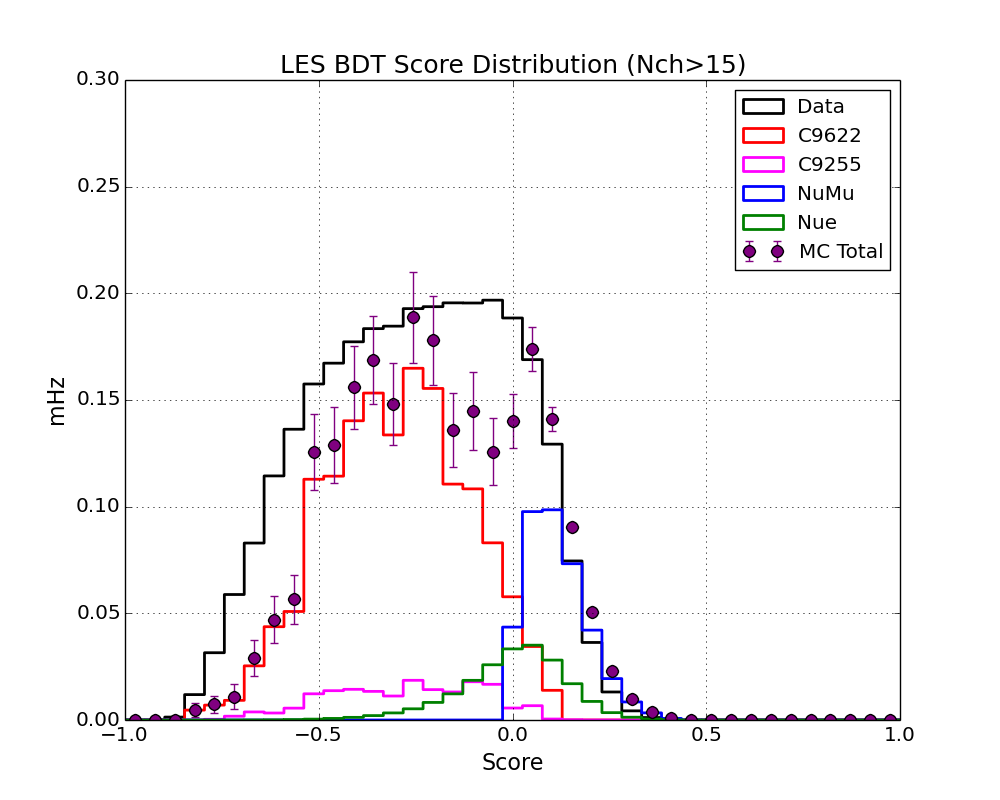
\includegraphics[width=0.5\textwidth,keepaspectratio]{plots/LES_BDTScoreDist_NormalizedRates_WC9255_And_H3AC9622_L6_NchCut_G1460.png}
  \end{center}
  \caption[Low-Energy Event Branch BDT Score Distribution]{[add caption]}
  \label{fig:LESBDTDistribution}
\end{figure}

\section{Analysis Method}
The search methods employed in the analysis of this data are nearly identical to those used in previous time-dependent IceCube analyses (see \cite{2008APh....29..299B} and \cite{2015arXiv150300598A}). The arrival times and directions of events within the dataset are fed to a likelihood function which is then used to perform a likelihood ratio test to compare a signal plus background hypothesis for the data to the background only hypothesis.

Construction of this likelihood function begins with the assignment of individual event probabilities that reflect the likelihood of seeing an event $i$ with arrival time $t_i$, reconstructed direction $\vec{x}_i$, and angular uncertainty $\sigma_i$ given a hypothetical source located at $\vec{x}_s$ with strength $n_s$ having a Gaussian time profile with mean time $t_0$ and width $\sigma_w$.
\begin{equation}\label{eq:EventProb}
\mathcal{P}_i(\vec{x}_i,t_i,\sigma_i|\vec{x}_s,n_s,t_0,\sigma_w) = \frac{n_s}{n_{\mathrm{tot}}} \mathcal{S}_i + \left(1-\frac{n_s}{n_{\mathrm{tot}}}\right) \mathcal{B}_i
\end{equation}
The $\mathcal{S}_i$ and $\mathcal{B}_i$ terms listed in Eq. \ref{eq:EventProb} are the signal and background probability density functions (p.d.f.) respectively. The p.d.f.s used in this search differ slightly from those in previously reported searches in that they use no reconstructed energy information. The signal p.d.f. is given by
\begin{equation}
\mathcal{S}_i(|\mathbf{x}_i-\mathbf{x}_s|,t_i,t_o,\sigma_w,\sigma_i) = S_i(|\mathbf{x}_i-\mathbf{x}_s|,\sigma_i) \cdot T_i(t_i,t_o,\sigma_w)
\end{equation}
where
\begin{equation}
S_i(|\mathbf{x}_i-\mathbf{x}_s|,\sigma_i) = \frac{\kappa}{4\pi \sinh \kappa} \exp \left(\kappa \cos |\mathbf{x}_i-\mathbf{x_s}|\right)
\end{equation}
and
\begin{equation}
T_i(t_i,t_o,\sigma_w) = \frac{1}{\sqrt{2\pi}\sigma_w} \exp \left(-\frac{(t_i-t_o)^2}{2 \sigma_w^2}\right)
\end{equation}
The spatial component of the signal p.d.f., $S_i$, features another difference with respect to previous searches (see \cite{2014ApJ...796..109A}). Due to the larger estimated error in reconstructed direction for low energy events, the Kent-Fisher distribution is used to model the probability of event-source association, and it is analogous to the Gaussian distribution normalized to the 2-sphere \citep{Fisher_Bingham}.

The background p.d.f., $\mathcal{B}_i$, is derived from the final level data set which is dominated by background. It has the following form
\begin{equation}
\mathcal{B}_i(\mathbf{x}_i,t_i) = P_{BkgDec}(\delta_i)\frac{P_{BkgAz}(\alpha_i)}{T}
\end{equation}
where $T$ is the total livetime of the search, $P_{BkgDec}(\delta_i)$ is a p.d.f. describing the event declination distribution, and $P_{BkgAz}(\alpha_i)$ is a p.d.f. describing the event distribution in detector azimuth. These p.d.f.s are generated directly from data and do not depend on any background simulation.

The likelihood function itself is simply the product sum of all individual event probabilities:
\begin{equation}\label{eq:LLH}
\mathcal{L}(\mathbf{x}_s,n_s,t_0,\sigma_w) = \prod \mathcal{P}_i(|\mathbf{x}_i-\mathbf{x}_s|,n_s,t_i,t_0,\sigma_w,\sigma_i)
\end{equation}
The ratio between the likelihood function values under the background only hypothesis ($n_s=0$) and the signal plus background hypothesis is maximized through variation of the source parameters $n_s$, $\sigma_w$, and $t_0$. The test statistic $\hat{\lambda}$ is then defined as the maximum value of the likelihood ratio:
\begin{equation}\label{eq:TS}
\hat{\lambda} = -2\log \left[\frac{\sqrt{2\pi}\hat{\sigma}_w}{T}\frac{\mathcal{L}(n_s = 0)}{\mathcal{L}(\vec{x}_s,\hat{n}_s,\hat{t}_o,\hat{\sigma}_w)} \right]
\end{equation}
with $\mathcal{L}(n_s = 0)$ corresponding to the likelihood of the null hypothesis and $\mathcal{L}(\vec{x}_s,{n}_s,\hat{t}_o,\hat{\sigma}_w)$ the likelihood of the signal plus background hypothesis with the best-fit values of the source parameters. Because this is a search for sources of finite duration over a timescale of limited duration, the number of potential short duration flares within the data set exceeds that of flares of longer duration leading to an effective trials factor. This results in a bias towards flares of shorter duration. We counteract this effect through the introduction of a marginalization term $T/\sqrt{2\pi}\hat{\sigma_w}$ in test statistic formulation which serves to penalize flares of shorter duration. More details about this term and its justification can be found in \cite{2010APh....33..175B}.

The test statistic is defined such that it will asymptotically follow a $\chi^2$ distribution with degrees of freedom corresponding to the number of fitted parameters for data consisting solely of background events. This enables the value of the maximized test statistic $\hat{\lambda}$ to be used to estimate the pre-trials p-value of the best-fit flare. Because this search attempts to look many times over the whole Northern sky, the actual significance of a given flare will need to be adjusted to account for the effective number of trials accrued during the sky scan. We use the procedure detailed in \cite{2015arXiv150300598A} that involves scrambling the event arrival times in the final dataset which also serves to scramble event right ascension. The search is performed on the randomized background data set and the p-value of the most significant flare in the search is recorded. Many iterations are performed to build a distribution of p-values which can then be compared to the p-value of the result from the real data. The fraction of background trials that result in a p-value of equal or greater significance than the observed p-value dictates the probability that the observed result is simply the consequence of a random background fluctuation. This probability is referred to as the post-trials p-value and it represents the true significance of the search result with proper trials factor correction.

In order to preserve generality, the presented search makes no use of information outside of the data set to designate source regions or time periods of interest. Instead, each point in the sky over a declination band ranging from -5$^{\circ}$ to 90$^{\circ}$ is examined. This is accomplished by discretizing the sky into separate bins and letting the location of these bins serve as the location of a hypothetical flaring source. Maximization of the likelihood is then performed at each bin to obtain a test statistic $\hat{\lambda}$ for each bin. The first iteration of this scan uses a relatively coarse 2$^{\circ}$ by 2$^{\circ}$ binning. Following completion of this first scan, a followup scan with finer 0.5$^{\circ}$ by 0.5$^{\circ}$ binning is performed over coarse bins featuring a pre-trials p-value more significant than a predefined threshold ($-\log_{10}($p-value$) > 1.75$). The result is a map of pre-trials p-values which shows the estimated significance of the best-fit flare hypothesis at each bin. The best-fit flare from the bin featuring the most significant maximized test statistic after both scans is returned as the hottest spot in the search.

\section{Results and Interpretations}
Applying the described analysis method on the unscrambled dataset yields the skymap of the pre-trials p-values shown in Figure \ref{fig:RealSkyMap}. The most significant flare is located at (RA, Dec.) = (268.75$^{\circ}$, 54.25$^{\circ}$) with a signal strength $n_s$ of 13.53 signal events and has a width $\sigma_w$ of 5.89 days with the peak occurring on MJD 56107 (2012 June 29). The pre-trials p-value for this flare is estimated at 6.68$\times 10^{-5}$. The post-trials probability of seeing such a flare from background only data is 56$\%$ indicating that this flare is entirely consistent with a background only explanation of the data.
\begin{figure}[ht]
  \begin{center}
    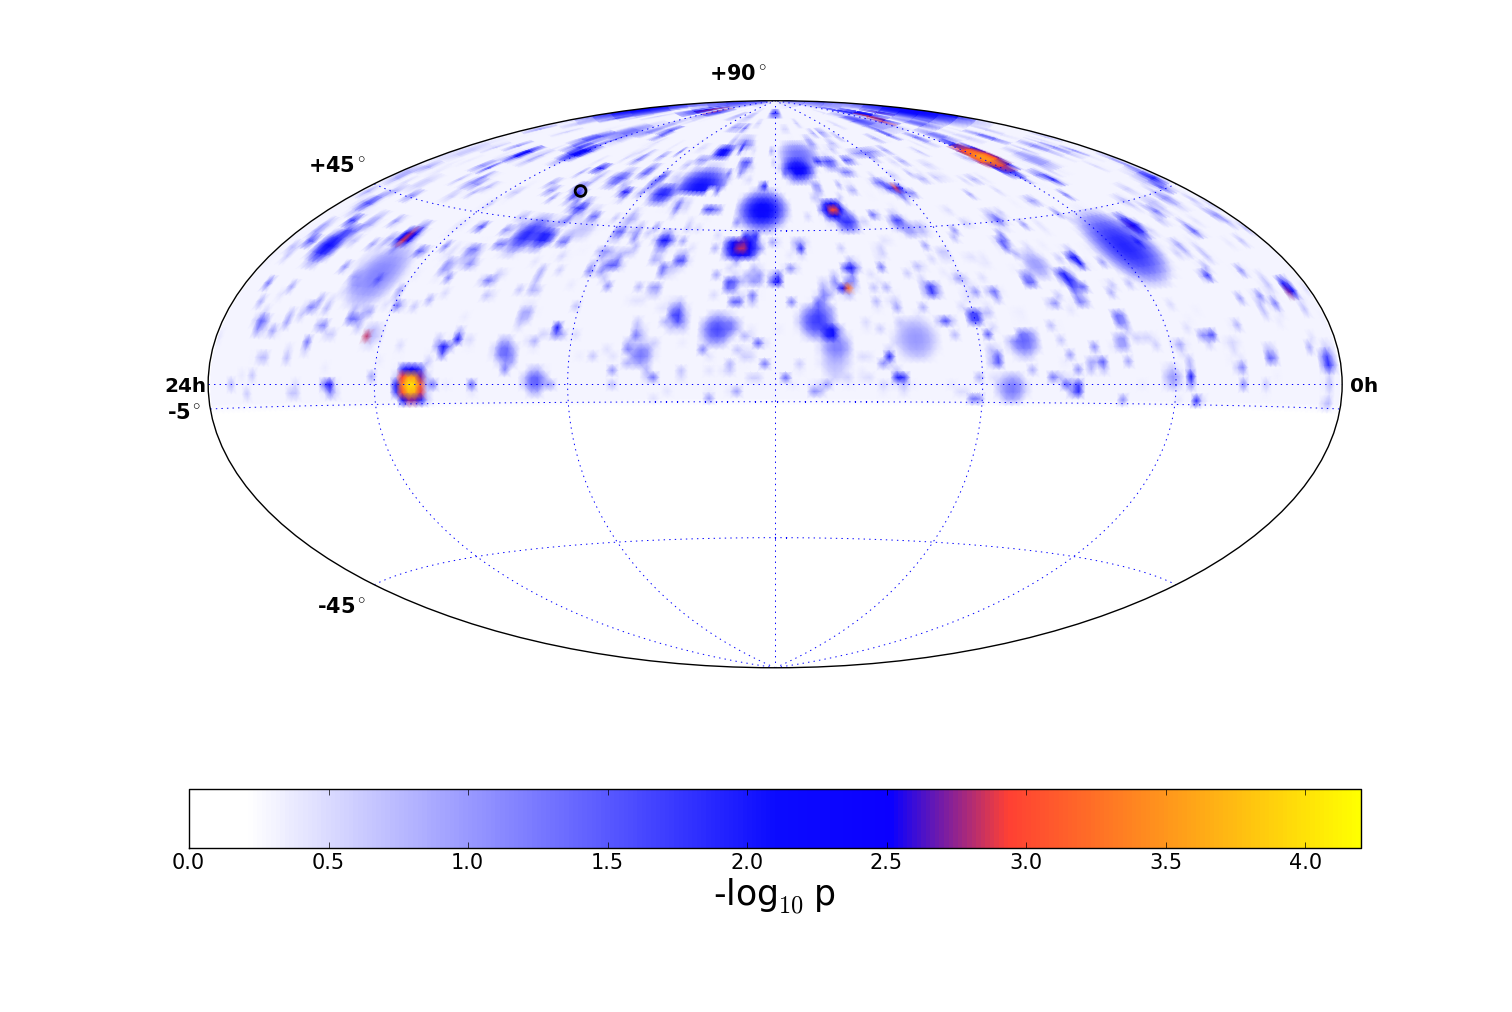
\includegraphics[width=1.0\textwidth,keepaspectratio]{plots/RealResultSkyMap.png}
  \end{center}
  \caption[Results Sky Map]{Sky map of pre-trials p-values for best fit flares per bin. The black circle identifies the location of the most significant flare found at RA = 268.75$^\circ$ and Declination = 54.25$^\circ$.}
  \label{fig:RealSkyMap}
\end{figure}
Given this null result, we can set an upper limit on the neutrino flux of any possible unobserved neutrino flare that may have occurred during the search period. Due to the focus on low-energy events in this search, we choose to examine the limit with respect to a soft-spectrum $E^{-3}$ generic flaring neutrino source with a Gaussian emission profile. An an upper limit is established through signal injections at a specified location. The background p-value distribution at the chosen location is constructed from several time scramblings of the data. Signal events are then injected with some Poisson mean value that is increased until the recovered p-values from the injections exceeds that of the median background p-value 90$\%$ of the time. This Poisson mean number of signal events is then taken as an event upper limit for the analysis method.

The upper limit for this generic flaring source for several emission timescales is plotted in Figure \ref{fig:GenericE3Limit}. The limit begins to rise precipitously at longer timescales as the rate of nearby background events becomes non-negligible. A limit on the time-integrated flux (GeV$^{-1} \cdot$ cm$^{-2}$) is plotted as well. This limit is obtained by folding the source spectrum with the effective area of the event selection and normalizing the flux so that the number of events produced in the detector corresponds to the calculated Poisson mean event upper limit.
%\begin{table}[h]
%\begin{center}
%\begin{tabular}{ccccccc}
%  \toprule
%R.A. &  Dec & $\hat{n}_s$ & $\hat{t}_0 [MJD]$ & $\hat{\sigma}_w [days]$ & p-value & p-value post-trial \\
%\midrule
%268.75$^{\circ}$ & 54.25$^{\circ}$ & 13.528 & 56107.8 & 5.89 & 4.1751 & 56$\%$\\
%\end{tabular}
%\caption[Best-fit signal parameters]{Best-fit values for flare location, %duration, strength and time.\label{tab:best_fit_flare}}
%\end{center}
%\end{table}

\begin{figure}[ht]
  \begin{center}
    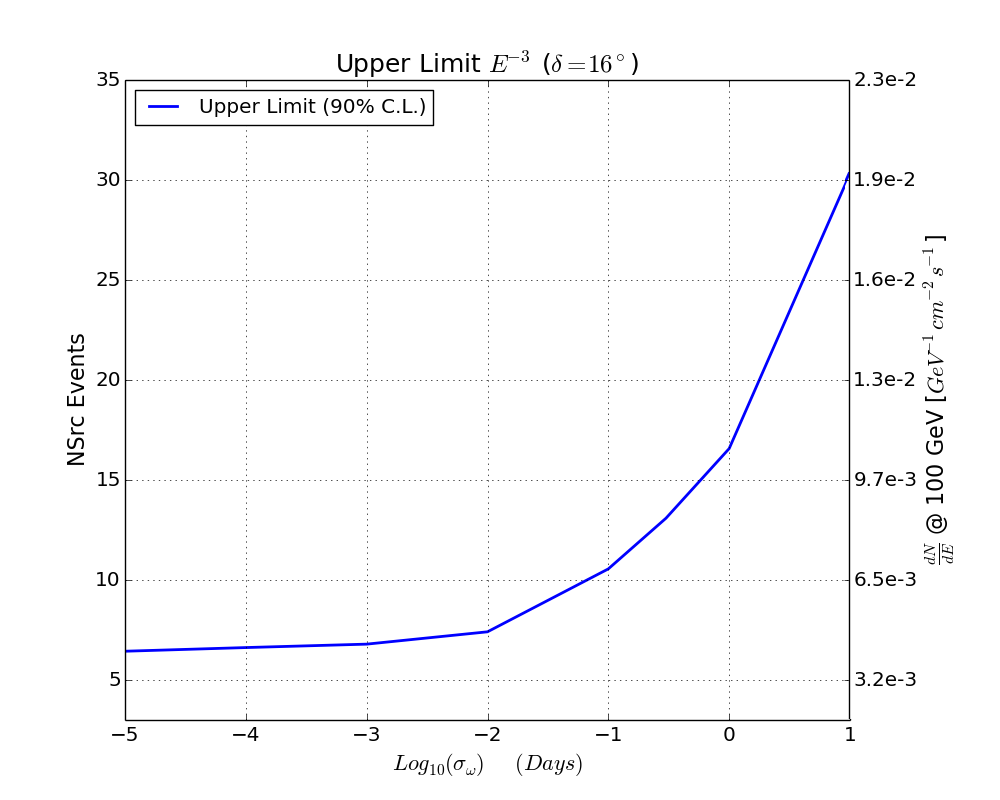
\includegraphics[width=1.0\textwidth,keepaspectratio]{plots/LowEnTransient_NEventSensitivity_E3_G1460_Dec16_DoubleY2.png}
  \end{center}
  \caption[Time-integrated Flux Limit for E$^{-3}$ Source]{Upper limit (90$\%$ C.L.) for a generic E$^{-3}$ transient source as a function of flare width $\sigma_w$.The limit is given in mean number of events (left axis) as well as in time-integrated flux at a reference energy of 100 GeV (right axis).}
  \label{fig:GenericE3Limit}
\end{figure}

\subsection{Choked GRB Limits}
This null result can also be used to construct limits on specific neutrino emission models such as the model for choked GRB emission by \cite{2004PhRvL..93r1101R} and \cite{2005PhRvL..95f1103A} mentioned previously in the introduction. Unlike the hard spectra sources (E$^{-2}$) that are the typical target in IceCube searches, the neutrino flux for choked GRBs is predicted to be much softer. The spectral shape can be modeled via a doubly broken power law with spectral breaks occurring as hadronic ($E_{nu^{(1)}}$) and radiative ($E_{nu^{(2)}}$) cooling mechanisms become efficient respectively (see Eq. \ref{eq:chkgrb_spec}). The fluence $F_\nu$ at Earth is given by Eq. \ref{eq:nuflu} and depends upon the pion (kaon) multiplicity $<n>$, neutrino production branching ratio for pions (kaons) $B_{\pi(K)}$, minimum and maximum proton energies ($E_{p,min}', E_{p,max}'$), kinetic energy of the jet $E_j$, bulk Lorentz factor $\Gamma_b$, and lastly the distance to the source $D$.
\begin{equation}\label{eq:chkgrb_spec}
\frac{d\Phi_\nu}{dE}=F_\nu\left\{\begin{array}{cc}
E^{-2} & E > E_{\nu}^{(1)} \\ 
E_{\nu}^{(1)}E^{-3} & E_{\nu}^{(1)}< E < E_{\nu}^{(2)} \\ 
E_{\nu}^{(1)}E_{\nu}^{(2)}E^{-4} & E_{\nu}^{(2)}< E < E_{max}
\end{array}\right.
\end{equation}
\begin{equation}\label{eq:nuflu}
F_{\nu} = \frac{<n>_{\pi(K)}B_{\pi(K)}}{8} \cdot \frac{E_j \Gamma_b^2}{2 \pi D^2 \textrm{ln}(E_{p,max}'/ E_{p,min}')}
\end{equation}



\begin{figure}[ht]
  \begin{center}
    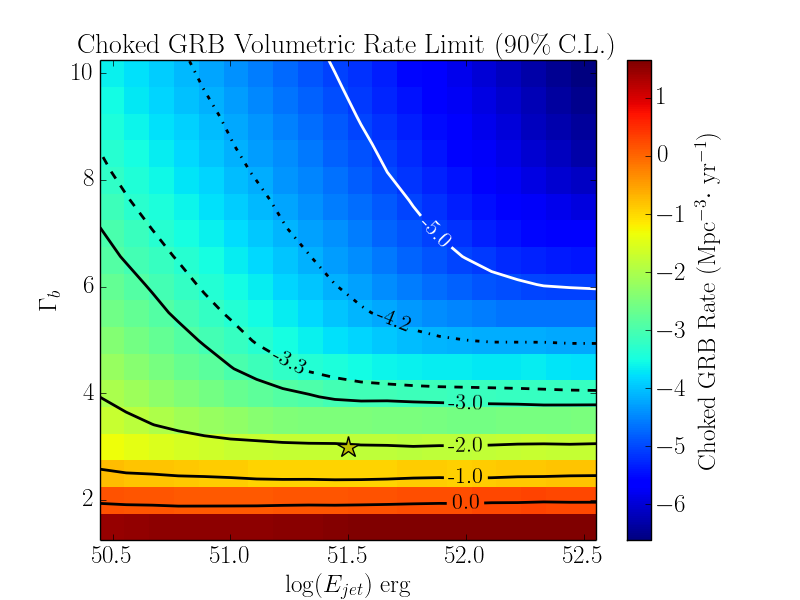
\includegraphics[width=1.0\textwidth,keepaspectratio]{plots/RateLimit_2DHisto_wContours_SysAdj.png}
  \end{center}
  \caption[Choked GRB Volumetric Rate Limit]{[add caption]}
  \label{fig:VolumetricRateLimit}
\end{figure}
\acknowledgments




\bibliography{IceCube_2012_LowEnTransient}{}

\clearpage

%% Use the figure environment and \plotone or \plottwo to include
%% figures and captions in your electronic submission.
%% To embed the sample graphics in
%% the file, uncomment the \plotone, \plottwo, and
%% \includegraphics commands
%%
%% If you need a layout that cannot be achieved with \plotone or
%% \plottwo, you can invoke the graphicx package directly with the
%% \includegraphics command or use \plotfiddle. For more information,
%% please see the tutorial on "Using Electronic Art with AASTeX" in the
%% documentation section at the AASTeX Web site, http://aastex.aas.org/
%%
%% The examples below also include sample markup for submission of
%% supplemental electronic materials. As always, be sure to check
%% the instructions to authors for the journal you are submitting to
%% for specific submissions guidelines as they vary from
%% journal to journal.

%% This example uses \plotone to include an EPS file scaled to
%% 80% of its natural size with \epsscale. Its caption
%% has been written to indicate that additional figure parts will be
%% available in the electronic journal.

%\begin{figure}
%\epsscale{.80}
%\plotone{f1.eps}
%\caption{Derived spectra for 3C138 \citep[see][]{heiles03}. Plots for all %sources are available
%in the electronic edition of {\it The Astrophysical Journal}.\label{fig1}}
%\end{figure}

\clearpage

%% Here we use \plottwo to present two versions of the same figure,
%% one in black and white for print the other in RGB color
%% for online presentation. Note that the caption indicates
%% that a color version of the figure will be available online.
%%

%\begin{figure}
%\plottwo{f2.eps}{f2_color.eps}
%\caption{A panel taken from Figure 2 of \citet{rudnick03}. 
%See the electronic edition of the Journal for a color version 
%of this figure.\label{fig2}}
%\end{figure}

%% This figure uses \includegraphics to scale and rotate the still frame
%% for an mpeg animation.

%\begin{figure}
%\includegraphics[angle=90,scale=.50]{f3.eps}
%\caption{Animation still frame taken from \citet{kim03}.
%This figure is also available as an mpeg
%animation in the electronic edition of the
%{\it Astrophysical Journal}.}
%\end{figure}

%% If you are not including electonic art with your submission, you may
%% mark up your captions using the \figcaption command. See the
%% User Guide for details.
%%
%% No more than seven \figcaption commands are allowed per page,
%% so if you have more than seven captions, insert a \clearpage
%% after every seventh one.

%% Tables should be submitted one per page, so put a \clearpage before
%% each one.

%% Two options are available to the author for producing tables:  the
%% deluxetable environment provided by the AASTeX package or the LaTeX
%% table environment.  Use of deluxetable is preferred.
%%

%% Three table samples follow, two marked up in the deluxetable environment,
%% one marked up as a LaTeX table.

%% In this first example, note that the \tabletypesize{}
%% command has been used to reduce the font size of the table.
%% We also use the \rotate command to rotate the table to
%% landscape orientation since it is very wide even at the
%% reduced font size.
%%
%% Note also that the \label command needs to be placed
%% inside the \tablecaption.

%% This table also includes a table comment indicating that the full
%% version will be available in machine-readable format in the electronic
%% edition.

\clearpage


\end{document}